% !TeX root = ../main.tex

\chapter{样本库的建立及数据分析}
特征提取需要大量样本才能提取出相对准确的信息,对于不同类型的数据也有不同的分析方法,
本章主要介绍研究过程中样本库的建立过程以及数据分析方法,流程图如图4.1所示。
\begin{figure}[htb]
    \centering
    
\includegraphics[width=\textwidth]{特征提取流程图.png}
    \caption{样本库的建立及数据分析流程图}
    %\label{fig:logo}
    %\note{注:图注的内容不宜放到图题中。}
\end{figure}

\section{云图数据的获取和分类}
本文数据全部来自于我国第二代静止气象卫星,风云四号气象卫星(FY4A星),该星装载多种观测仪器,
包括多通道扫描成像辐射计、闪电成像仪、空间环境监测仪器和干涉式大气垂直探测仪等仪器。
FY4A提供各个观测仪器的L1级数据,包括成像仪500M,1KM,2KM,4KM等不同分辨率全圆盘数据,
闪电仪1分钟组产品等。FY4A还提供了32种定量产品,包括云和大气产品、地表类产品、天气产品、
辐射产品等多种种类,大气的相关信息可以由大气类产品来监测,环境监测主要用地表类产品,
环境灾害天气的监测则主要使用天气类产品,地气系统辐射收支情况则用辐射类产品来反映。

本文实验数据来自于中国气象局国家卫星气象中心,可通过风云卫星遥感数据服务网下载卫星数据。
经过分析比较最终选取了成像仪全圆盘4KML1数据,闪电仪1分钟组产品和云检测实时产品,
其中成像仪全圆盘4KML1数据用于提取$0.45\sim13.8\mu m$等14个通道的云图数据,
闪电仪1分钟组产品用于建立雷暴云数据库,云检测实时产品用于建立非雷暴云数据库。

在风云卫星遥感数据服务网选取数据提交订单后,由国家气象卫星中心回调所需数据,
回调完成将返回下载数据所需的用户名和密码,在个人服务器端通过FTP即可进行下载。
下载完成后的成像仪全圆盘数据为HDF格式,闪电仪组产品和云检测产品为NC格式,为方便后续处理,
根据文件名将不同数据分类保存至对应文件夹。成像仪和云检测产品的数据以一小时为间隔,
闪电仪的数据以一分钟为间隔,为了将闪电仪数据和成像仪数据相匹配,
本文选取成像仪数据时间后十分钟闪电仪数据,
保存至对应文件件。分类后的文件格式如图4.2:
\begin{figure}[htb]
    \centering
    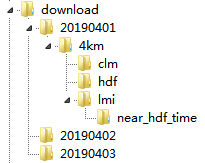
\includegraphics[width=0.4\textwidth]{分类后文件格式.png}
    \caption{分类后文件格式}
    %\label{fig:logo}
    %\note{注:图注的内容不宜放到图题中。}
\end{figure}

其中download表示下载的数据,下级目录20190401表明数据时间,下级目录4km表明数据分辨率为4km,
其中clm中存放云检测产品数据,hdf中存放成像仪全圆盘数据,lmi中存放闪电仪数据,
near$\_$hdf$\_$time文件夹单独存放临近成像仪数据时间的闪电仪数据。


\section{样本库的建立}
本文需要分析大量分析,才能得出相对准确的结果,因此样本库的建立是非常重要的一步,将根据闪电仪数据和
云检测产品建立雷暴云样本库和非雷暴云样本库,为之后的特征提取分析奠定基础。

\subsection{雷暴云样本库的建立}
雷暴云样本库的建立需要闪电仪数据作为已知信息,闪电成像仪是全球第一批两颗静止气象卫星闪电成像仪之一,
我国首次研制,采用CCD面阵和光学成像技术,对观测区域内包括云闪、云间闪、云地闪在内的总闪电进行凝视观测,
实现对雷暴系统的实时、连续监测和跟踪。数据以NC格式存储,其中存储着一次闪电事件的经纬度,辐射强度,
发生时间等信息,为方便后续处理,提取所有闪电信息并保存为csv文件,文件如图4.3所示:

\begin{figure}[htb]
    \centering
    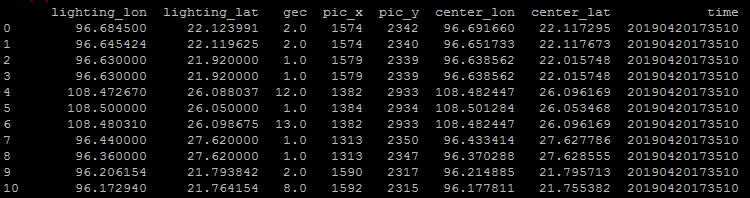
\includegraphics[width=\textwidth]{存储闪电信息的csv文件.png}
    \caption{存储闪电信息的csv文件}
    %\label{fig:logo}
    %\note{注:图注的内容不宜放到图题中。}
\end{figure}


每一行表示一次闪电事件,lighting$\_$lon表示闪电实际发生的经度,lighting$\_$lat表示闪电实际发生的纬度,
gec表示闪电的强度(标准化后的数值,与实际闪电辐射强度成正比),pic$\_$x,pic$\_$y,center$\_$lon,center$\_$lat
分别表示闪电对应在hdf卫星云图上的行列值,以及对应的经纬度
(由于hdf云图中没有经纬度数据,只能通过官方文档《FY-4A数据行列号和经纬度查找表4km》查表计算),
time表示闪电发生的时间,依次为年月日时分秒。

根据闪电仪csv中数据即可从成像仪hdf数据中提取出各通道对应的卫星云图,
首先根据time闪电时间信息找到对应时间的hdf数据,接着根据pic$\_$x和pic$\_$y即闪电对应hdf数据行列号,
设置不同分辨率(以行列号为中心)即可提取出不同通道的雷暴云图像。最终生成的文件树如图4.4。

\begin{figure}[htb]
    \centering
    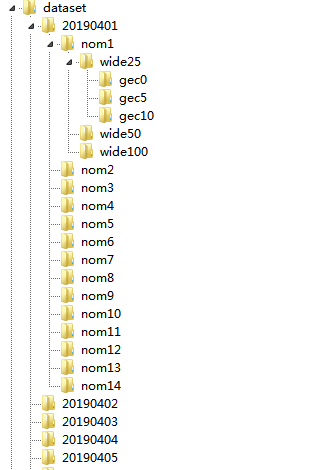
\includegraphics[height=0.5\textwidth]{雷暴云数据库文件格式.png}
    \caption{雷暴云数据库文件格式}
    %\label{fig:logo}
    %\note{注:图注的内容不宜放到图题中。}
\end{figure}

dataset表示数据库,20190401表示数据库年月日,nom1~14表示全圆盘4KM数据14个通道数据
,$wide25$,$wide50$,$wide100$表示生成云图的分辨率(即像素值),
gec5表示雷暴强度为$5\sim10$的数据集,gec10表示雷暴强度为$10\sim15$的数据集。

根据官方文档可知,云图数据以辐射值存储,变化范围为0$\sim$65534,其中65535为无效值,
因此在处理时,将65535变为0,将0$\sim$65535压缩到0$\sim$255,调用opencv相关函数生成云图图像。
生成的雷暴云图如图4.5。


\iffalse
\begin{figure}[htb]
\centering
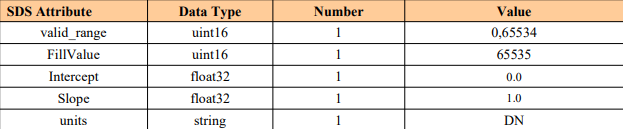
\includegraphics[width=\textwidth]{云图图像数据层数据官方文档.png}
\caption{云图图像数据层数据官方文档}
%\label{fig:logo}
%\note{注:图注的内容不宜放到图题中。}
\end{figure}
\fi


\begin{figure}[htb]
    \centering
    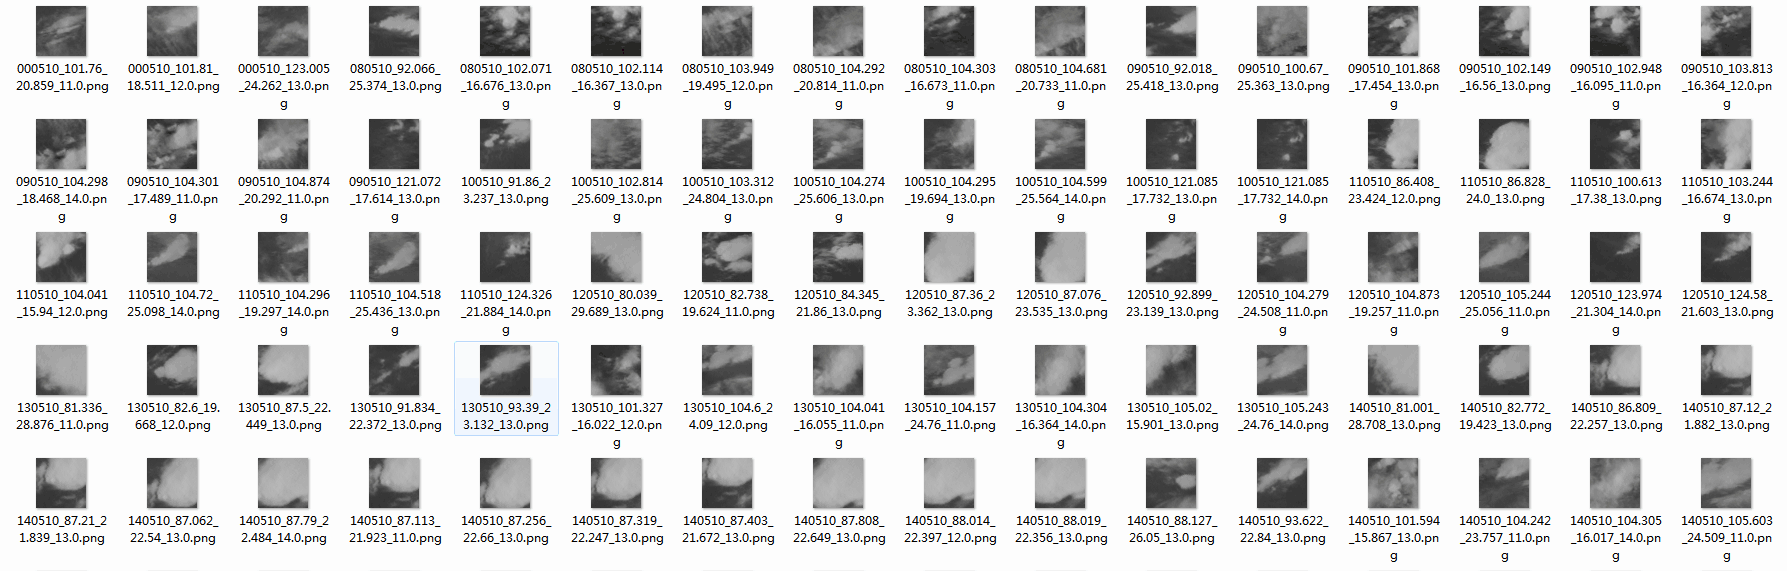
\includegraphics[width=\textwidth]{生成的雷暴云图像2.png}
    \caption{生成的雷暴云图像}
    %\label{fig:logo}
    %\note{注:图注的内容不宜放到图题中。}
\end{figure}


\subsection{非雷暴云样本库的建立}
非雷暴云样本库的建立需要云检测产品作为已知信息,风云四号云检测产品处理是联合利用多通道
扫描成像仪的多个通道,采用阈值法,经过处理,生成的云检测产品。云检测产品中填充值0表示为云,1表示可能为云,2表示可能晴空,3表示晴空,126表示地表之外的空间,127表示无效值。
不同分辨率下某一区域平均值小于一定阈值,即可将此区域判定为云,
选取示意图如图4.6所示。
\begin{figure}[htb]
    \centering
    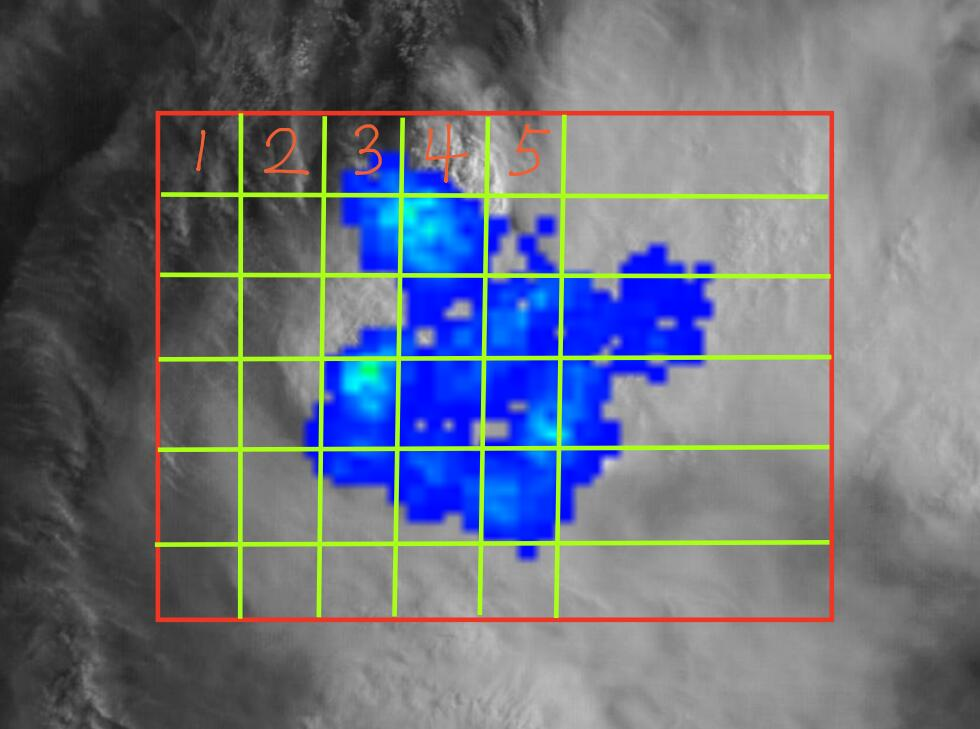
\includegraphics[height=0.5 \textwidth]{非雷暴区域选定示意图.jpg}
    \caption{非雷暴区域选定示意图}
    %\label{fig:logo}
    %\note{注:图注的内容不宜放到图题中。}
\end{figure}



以一定分辨率划定区域,本文假定划定区域平均值小于0.01即判断为云,
则此实例中1,2判定为非云区,3,4,5区域可判定为云区,其中3,4区域由于有闪电仪数据,
因此只有5区域判定为非云区,
将生成的云图图像保存至对应通道对应分辨率的gec0文件夹中,表示雷暴强度为0。
生成的部分非雷暴云图如图4.7。文件名分别表示时间和经纬度。
\begin{figure}[htb]
    \centering
    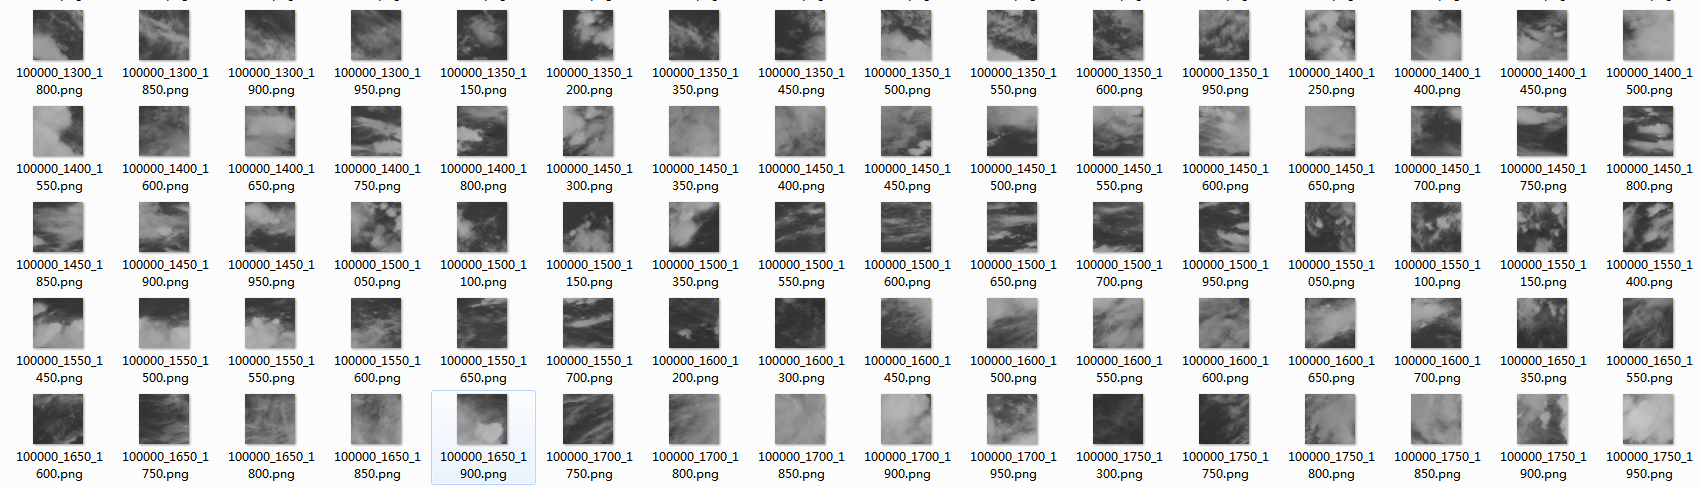
\includegraphics[width=\textwidth]{部分非雷暴云图.png}
    \caption{部分非雷暴云图}
    %\label{fig:logo}
    %\note{注:图注的内容不宜放到图题中。}
\end{figure}


\section{图像的特征提取}

\subsection{纹理特征提取}
本文采用灰度共生矩阵的方法对图像的纹理特征进行计算,
挑选了ASM,CON,IDM,ENG等四个量值进行图像的分类。
如果影像中噪声越多,则ASM能量值就越小,代表影像纹理越丰富。
如果影像中地物灰度分布均匀(例如,云层、水体),则ASM能量值越大,纹理信息越弱。
对比度(CON)描述的是影像中像素与其周围像素的反差对比。
对比度越小,说明该区域的像素灰度越均匀,纹理越弱,反之,纹理越丰富。
IDM是反映图像中某一区域内像元值变化程度的量。IDM值越大,说明图像中该区域的纹理越弱,
反之,纹理越丰富。熵原本用来描述分子不规则运动剧烈程度的物理量,
后来用来度量影像中所包含的纹理信息。熵值越大,说明影像中所包含的纹理信息越丰富,
反之,纹理信息越弱。计算得到的四种纹理特征量值如图4.8所示。

\begin{figure}[htb]
    \centering
    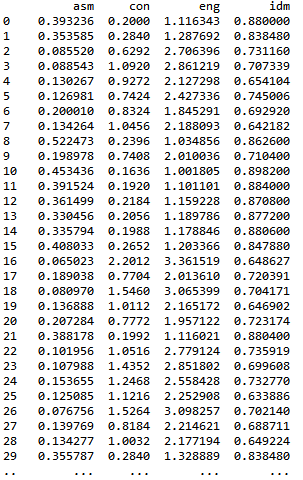
\includegraphics[width=0.5\textwidth]{计算得到的纹理特征量值.png}
    \caption{计算得到的纹理特征量值csv存储方式}
    %\label{fig:logo}
    %\note{注:图注的内容不宜放到图题中。}
\end{figure}

\iffalse
\begin{algorithm}[htb]
    \small
    \SetAlgoLined
    \KwData{this text}
    \KwResult{how to write algorithm}
  
    initialization\;
    \While{not at end of this document}{
      read current\;
      \eIf{understand}{
        go to next section\;
        current section becomes this one\;
      }{
        go back to the beginning of current section\;
      }
    }
    \caption{纹理特征计算算法}
    \label{algo:algorithm1}
\end{algorithm}
\fi

\newpage
\subsection{几何特征提取}
卫星云图上的各类云系都具有一定的边界形状,云的边界是判断天气系统的重要依据,如成熟的台风呈圆形,
冷锋云带呈气旋形弯曲。形状的描述主要分为以下几种方法:基于面积、伸长度、主轴方向等传统的形状特征;
基于形状变换的方法;基于形状相互关系的方法。本文主要从图形的周长,面积,等效直径,离心率等方面来描述形状特征。

首先通过阈值法提取出云图的二值图像,之后通过形态学的方法计算出图像的连通区域,不同区域标记为不同的颜色,
如图4.9所示。
\begin{figure}[htb]
    \centering
    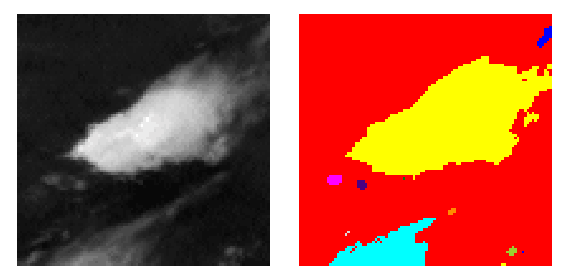
\includegraphics[width=0.9\textwidth]{阈值法处理后的云图区域.png}
    \caption{阈值法处理后的云图区域}
    %\label{fig:logo}
    %\note{注:图注的内容不宜放到图题中。}
\end{figure}
此图共提取出12块连通区域,可看出标记为黄色的连通区域表示此图中主要的云图信息,因此只需保留此块区域的几何特征,
通过计算各连通区域的面积,得出最大面积的连通区域即为此区域,计算此区域不同的几何特征,
将计算后的几何特征以csv的格式保存,如图4.10所示。
\begin{figure}[htb]
    \centering
    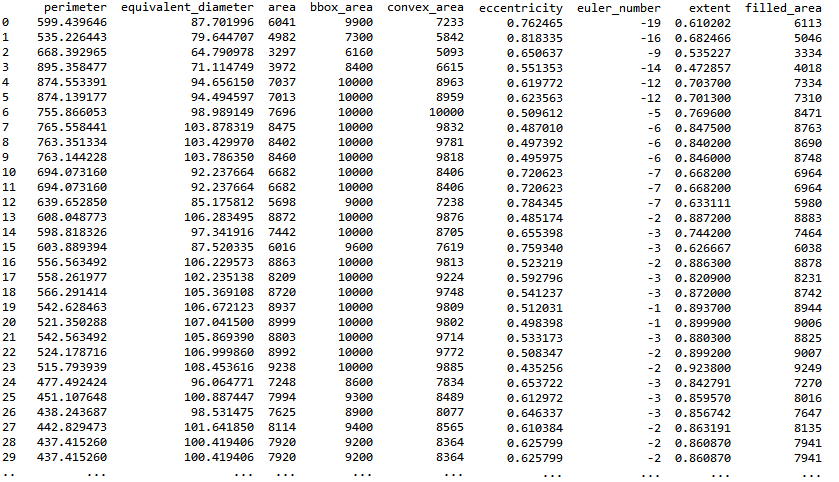
\includegraphics[width=\textwidth]{计算得到的几何特征.png}
    \caption{计算得到的几何特征csv存储方式}
    %\label{fig:logo}
    %\note{注:图注的内容不宜放到图题中。}
\end{figure}

perimeter表示区域周长,equivalent$\_$diameter表示等效直径(和区域面积相同的
圆的直径),area表示区域面积,bbox$\_$area表示边界外接框的面积,convex$\_$area表示凸包的
面积,eccentricity表示离心率,euler$\_$number表示欧拉数,extent表示区域面积和边界外接框面积的比率,
filled$\_$area区域和外接框之间填充的面积。

\iffalse
\subsection{频率特征提取}
影像频率是描述影像中光谱信息变化程度的的物理量。对于影像中的云层而言,
云层边缘灰度突变,因此分布在高频部分,
而云层内部灰度均匀,因此分布在低频部分。频率域为评价影像提供了一个全新的角度。
本文通过快速傅里叶变换,计算得出云图图像的幅度谱如图。

\begin{figure}[htb]
    \centering
    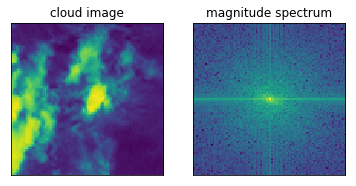
\includegraphics[width=0.5\textwidth]{卫星云图和FFT变换后的幅度谱.png}
    \caption{卫星云图和FFT变换后的幅度谱}
    %\label{fig:logo}
    %\note{注:图注的内容不宜放到图题中。}
\end{figure}
\fi


\section{特征数据的分析}
\subsection{纹理特征的分析}
4.3.1中提取到的ASM,CON,IDM,ENG等四个量值以CSV格式保存,由于数据维度并不高,不必采用主成分分析的方法
降维处理,在分析时通过比较不同分辨率,
不同雷暴强度 ,不同波段,不同的纹理特征组合,确定出区分雷暴云和非雷暴云的阈值范围,
主要采用散点图的方式进行数据可视化,x轴表示其中一种纹理特征值,y轴表示另一种纹理特征值,
将要比较的两幅图像叠加在一幅图像上,即可较为清晰的看出是否具有可靠的区分度。

第一幅图表示1通道分辨率为25像素雷暴强度为5以及1通道分辨率为50像素雷暴强度为5的asm值和con值的组合,
可看出不同分辨率的图像区分度并不高。第二幅图表示10通道分辨率为25像素雷暴强度为0(即非雷暴区域)
以及10通道分辨率为25像素雷暴强度为10的eng值和idm值的组合,具有较高的区分度。
关于纹理特征的详细分析,将重点在第五章进行讨论。

\begin{figure}[htbp]
\centering
\begin{minipage}[t]{0.48\textwidth}
\centering
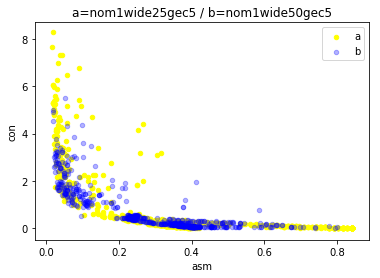
\includegraphics[width=6cm]{纹理特征分析方法1.png}
\caption{纹理特征分析方法1}
\end{minipage}
\begin{minipage}[t]{0.48\textwidth}
\centering
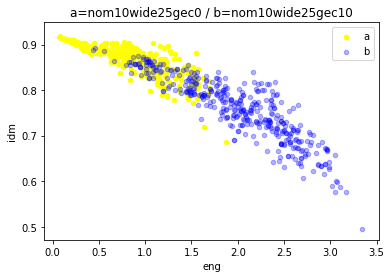
\includegraphics[width=6cm]{纹理特征分析方法2.png}
\caption{纹理特征分析方法2}
\end{minipage}
\end{figure}
    
\subsection{几何特征的分析}
\subsubsection{主成分分析方法}
4.3.2中提取到的纹理特征,共有周长、直径、面积等九个数据维度,
在分析时采用主成分分析的方法来降低数据维度。
主成分分析主要分为以下几步:

(1)对数据进行标准化处理;

(2)计算标准化后的协方差矩阵;

(3)计算协方差矩阵的特征值及特征向量;

(4)各成分贡献率并按大小排列;

(5)根据主成份贡献率的大小选取前m个主成份;

(6)将原始数据与对应的特征向量矩阵相乘即可得到降维后的数据。

经过计算得出的各分量贡献率如表4.1所示。

\begin{table}[htb]
    \centering\small
    \caption{主成分分析各分量贡献率}
    \label{tab:exampletable}
    \begin{tabular}{cllll}
      \toprule
        component & value & difference  & proportion & cumulative    \\
      \midrule
      1 & 6.3139 & 4.5995 & 0.7015 & 0.7015 \\
      2 & 1.7143 & 1.2567 & 0.1904 & 0.8920 \\
      3 & 0.4575 & 0.0877 & 0.0508 & 0.9428 \\
      4 & 0.3698 & 0.2487 & 0.0411 & 0.9839 \\
      5 & 0.1211 & 0.1083 & 0.1346 & 0.9974 \\
      6 & 0.0128 & 0.0039 & 0.0014 & 0.9988 \\
      7 & 0.0089 & 0.0077 & 0.0009 & 0.9998 \\
      8 & 0.0011 & 0.0007 & 0.0001 & 0.9999 \\
      9 & 0.0004 & 0 & 0.0001 &  1\\
      \bottomrule
    \end{tabular}
  \end{table}

由表4.1可以看出1,2分量累积贡献率已接近90$\%$,由1,2分量对应的特征向量
构成的特征矩阵,可以计算得出降维后的数据。由于采用了两个分量,
因此可以采用散点图的方式来表示数据,将雷暴云和非雷暴云的几何特征
降维后放在一张散点图中如图4.13所示。

\begin{figure}[htb]
    \centering
    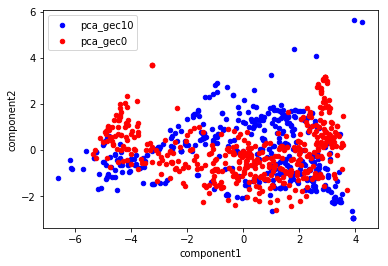
\includegraphics[width=0.8\textwidth]{降维后的几何特征分析.png}
    \caption{降维后的几何特征分析}
    %\label{fig:logo}
    %\note{注:图注的内容不宜放到图题中。}
\end{figure}

\subsubsection{密度图分析方法}
将计算出的不同的几何特征值用密度图来表示,可以看出不同特征值大致的分布,
每幅图下方标明此图对比的几何特征名称,
蓝色的线表示雷暴强度大于10的雷暴云对应的密度曲线,
红色的线表示非雷暴云对应的密度曲线。如图4.14所示。
\begin{figure}
    \centering
    \subfigure{
    \begin{minipage}[t]{0.25\linewidth}
    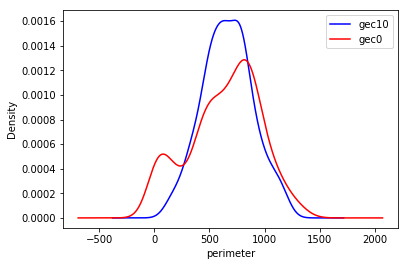
\includegraphics[width=1\linewidth,height=0.7\linewidth]{311.png}\vspace{2pt}
    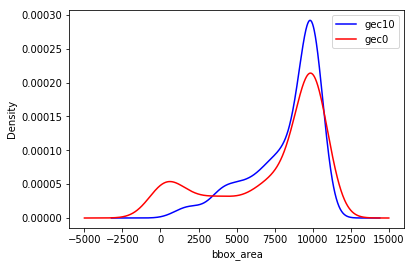
\includegraphics[width=1\linewidth,height=0.7\linewidth]{314.png}\vspace{2pt}
    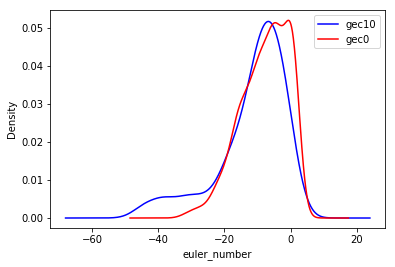
\includegraphics[width=1\linewidth,height=0.7\linewidth]{317.png}
    \end{minipage}}
    \subfigure{
    \begin{minipage}[t]{0.25\linewidth}
    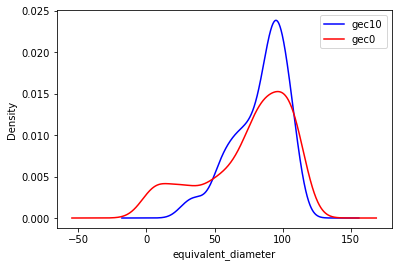
\includegraphics[width=1\linewidth,height=0.7\linewidth]{312.png}\vspace{2pt}
    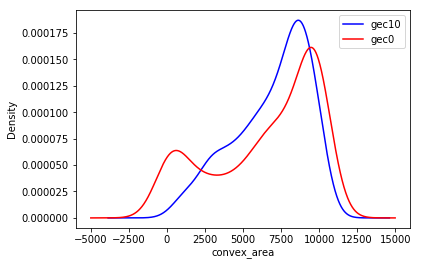
\includegraphics[width=1\linewidth,height=0.7\linewidth]{315.png}\vspace{2pt}
    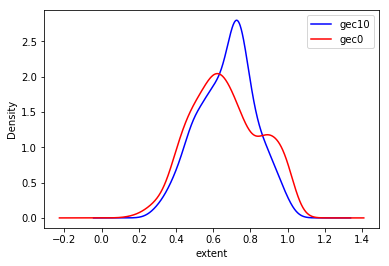
\includegraphics[width=1\linewidth,height=0.7\linewidth]{318.png}
    \end{minipage}}
    \subfigure{
    \begin{minipage}[t]{0.25\linewidth}
    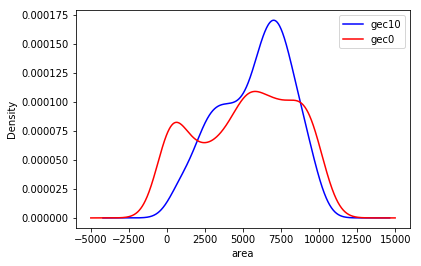
\includegraphics[width=1\linewidth,height=0.7\linewidth]{313.png}\vspace{2pt}
    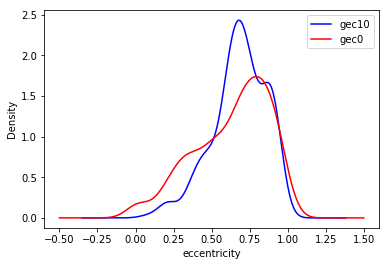
\includegraphics[width=1\linewidth,height=0.7\linewidth]{316.png}\vspace{2pt}
    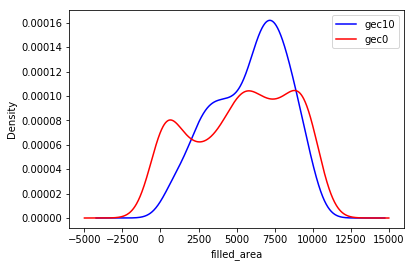
\includegraphics[width=1\linewidth,height=0.7\linewidth]{319.png}
    \end{minipage}}
    \caption{不同几何值的密度图}
    \end{figure}

perimeter表示区域周长,equivalent$\_$diameter表示等效直径(和区域面积相同的
圆的直径),area表示区域面积,bbox$\_$area表示边界外接框的面积,convex$\_$area表示凸包的
面积,eccentricity表示离心率,euler$\_$number表示欧拉数,extent表示区域面积和边界外接框面积的比率,
filled$\_$area区域和外接框之间填充的面积。
可以看出雷暴云和非雷暴云在各个特征值下,分布都非常接近,不能准确区分雷暴云和非雷暴云。

\section{测试库的建立和验证}
测试库的建立与样本库的建立方法类似,将提取到的雷暴云和非雷暴云放在一个文件夹中。
根据本文提出的图像特征阈值提取方法进行判别,为了对该方法进行定量化分析,
研究中引入了预警率、虚警率以及错误率为定量化标准,计算方法如下:
\begin{equation}
    PR=\frac{LC}{LC+CC}
\end{equation}
\begin{equation}
    CR=\frac{CC}{LC+CC}
\end{equation}
\begin{equation}
    ER=\frac{LI-LC}{LI}
\end{equation}
式中,$PR$为预警率,$LC$为识别出的雷暴云的数量,$CC$为识别出的非雷暴云的数量;
$CR$为虚警率;$ER$表示漏判率,$LI$表示测试库中雷暴云数量。 